\documentclass{beamer}
% Copyright 2015 by Do Phan Thuan

% Loại mẫu slice
%\usetheme{AnnArbor}
%\usetheme{Antibes}
\usetheme{Boadilla}
%\usetheme{CambridgeUS}
%\usetheme{Hannover}

% Ký tự tiếng Việt
\usepackage[utf8]{vietnam}
\usepackage[utf8]{inputenc}
\usepackage{alltt}
% Công thức toán
\usepackage{amsmath,amsthm,amssymb,epsfig}
% Chèn ảnh
\usepackage{graphicx}
% Chèn đường dẫn 
\usepackage{url}

% Vẽ đồ thị
\usepackage{pgfplots}

% Insert code
\usepackage{listings}
\usepackage{colortbl}


\usepackage{color}

\definecolor{dkgreen}{rgb}{0,0.6,0}
\definecolor{gray}{rgb}{0.5,0.5,0.5}
\definecolor{mauve}{rgb}{0.58,0,0.82}
  
\definecolor{Xanh}{rgb}{0,0.5,1}
\definecolor{Do}{rgb}{1,0.25,0}
\definecolor{Vang}{rgb}{1,1,0}
\definecolor{Datroi}{rgb}{0,0,1}


% multirow
\usepackage{multirow}

\usepackage{pbox}

% Tô mầu cho bảng
\usepackage{colortbl}
\definecolor{Xanh}{rgb}{0,0.5,1}
\definecolor{Do}{rgb}{1,0.25,0}
\definecolor{Vang}{rgb}{1,1,0}
\definecolor{Datroi}{rgb}{0,0,1}

% Một vài ký hiệu thường dùng
\def\R{{\mathbb R}}
\def\N{{\mathbb N}}
\def\X{{\mathcal X}}
\def\Y{{\mathcal Y}}
\def\F{{\mathcal F}}
\def\P{{\mathcal P}}
\def\E{{\mathbb E}}
\def\I{{\mathbb I}}
\def\sign{{\rm sign}}

% Xác định khoảng dãn trong bảng
\renewcommand\arraystretch{1.2}

% a few macros
\newcommand{\bi}{\begin{itemize}}
\newcommand{\ei}{\end{itemize}}
\newcommand{\ig}{\includegraphics}
\newcommand{\subt}[1]{{\footnotesize \color{subtitle} {#1}}}

% named colors
\definecolor{offwhite}{RGB}{249,242,215}
\definecolor{foreground}{RGB}{255,255,255}
\definecolor{background}{RGB}{24,24,24}
\definecolor{title}{RGB}{107,174,214}
\definecolor{gray}{RGB}{155,155,155}
\definecolor{subtitle}{RGB}{102,255,204}
\definecolor{hilight}{RGB}{22,155,104}
\definecolor{vhilight}{RGB}{255,111,207}
\definecolor{lolight}{RGB}{155,155,155}
%\definecolor{green}{RGB}{125,250,125}

% Minted
%\usepackage{minted}
%\usemintedstyle{monokai}
%\newminted{cpp}{fontsize=\footnotesize}


%gets rid of bottom navigation bars
\setbeamertemplate{footline}[frame number]{}

%gets rid of bottom navigation symbols
%\setbeamertemplate{navigation symbols}{}

%gets rid of footer
%will override 'frame number' instruction above
%comment out to revert to previous/default definitions
%\setbeamertemplate{footline}{}

% Tác giả, Tiêu đề, vân vân
\title[]{{\bf \large HyperLogLog in Practice: Algorithmic Engineering of a
State of The Art Cardinality Estimation Algorithm } \\
}
\author[]{
Nguyễn Tuấn Đạt \\% \inst{1} 
Đặng Quang Trung% \inst{1} 
}

\institute[]{
%\inst{1}% 

}

\logo{
\includegraphics[scale=0.05]{hust.jpg} \vspace{220pt}}

\begin{document}

\begin{frame}
\titlepage
\end{frame}

\begin{frame}{Nội dung}
\tableofcontents
\end{frame}
\section{Giới thiệu}

\begin{frame}{Giới thiệu bài toán Cardinality estimation}
\subsection{Cardinality estimation}
Là bài toán xác định số lượng phần tử khác nhau trong một data stream. 

Các yêu cầu :
\begin{itemize}
\item Accuracy ( Độ chính xác )
\item Memory efficiency ( Hiệu quả sử dụng bộ nhớ )
\item Estimate large cardinalities ( Ước lượng một tập rộng )
\item Practicality ( Tính thực tế )
\end{itemize}

\end{frame}
\begin{frame}
\color{hilight} Bài toán: 
\begin{itemize}
\item Input: Dãy S
\item Output: Ước lượng số phần tử khác nhau của S
\end{itemize}
\end{frame}
\subsection{Thuật toán HyperLogLog}
\begin{frame}{Thuật toán HyperLogLog}
\begin{itemize}
\item Hàm băm h : D -> $\{0,1\}^{32}$ 
\item Ta băm lần lượt từng phần tử trong S $$\forall x \in S,  h_x = h(x)  $$, ta được tập HX
Dựa vào p bit đầu của giá trị băm $p \in [4..16] $ ta sẽ chia HX thành m dãy con $HX_i$ bằng cách dựa vào p bit đầu của giá trị băm($m=2^p$) 

Với mỗi $HX_i$ số lượng số 0 liên tiếp đầu tiên lớn nhất trong các giá trị băm cộng một ( không tính p bit đã đã dùng để tách dãy ) sẽ được lưu vào mảng M, $ M[i] $ tương ứng với $HX_i$
$$ M[i]=max_{x \in HX} \varrho(x)  $$ với $\varrho $ số lượng số 0 liên tiếp đầu tiên lớn nhất trong các giá trị băm cộng một.
\end{itemize}
\end{frame}
\begin{frame}
Số lượng phần tử khác nhau trong đầu vào dãy S sẽ được ước lượng bằng công thức:
$$ E:= \alpha_m .m^2.(\sum_{j=1}^m 2^{-M[j]} )^{-1}$$ với $$ \alpha_m :=(m \displaystyle \int_0^\infty  (log_2 (\dfrac{2+u}{1+u})^m du)^{-1} ) $$
\end{frame}
\begin{frame}{Mô tả}
\begin{figure}[H]
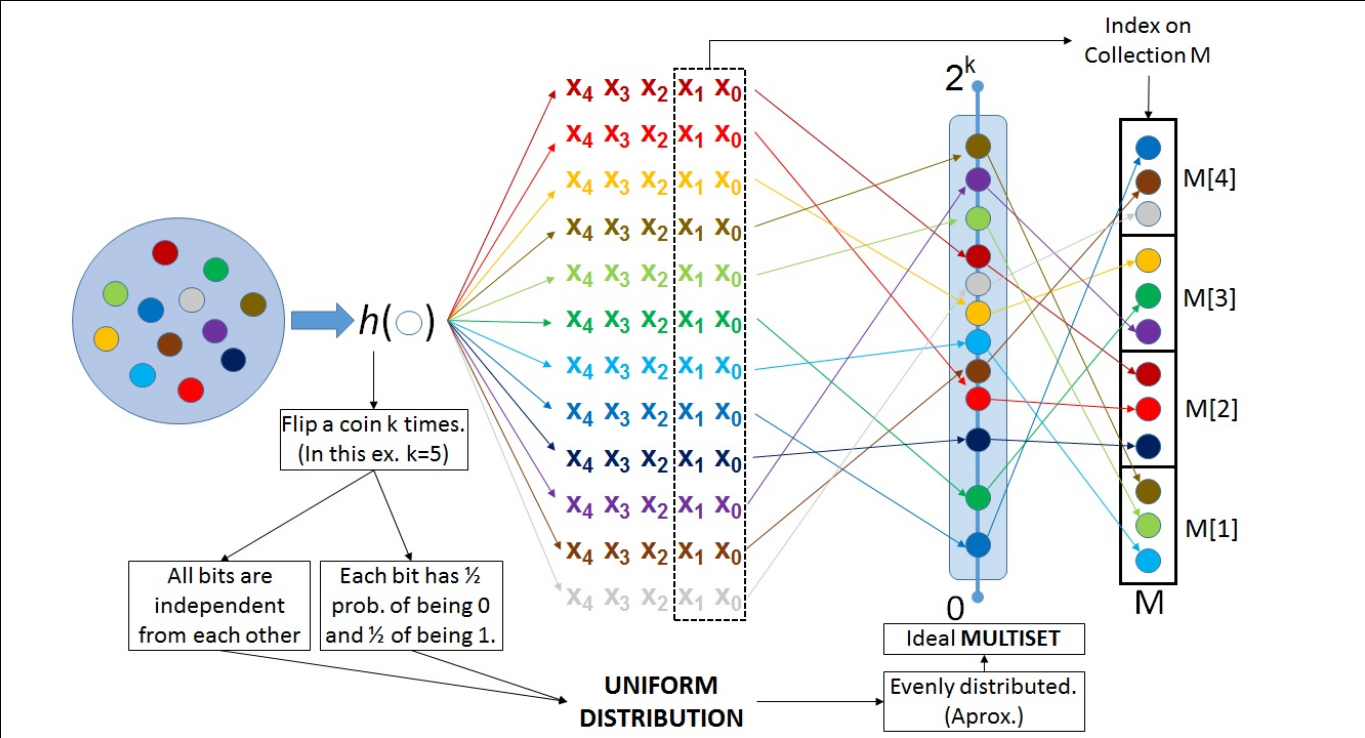
\includegraphics[scale=0.3]{HLL.png}

\end{figure}

\end{frame}
\begin{frame}
\begin{figure}[H]
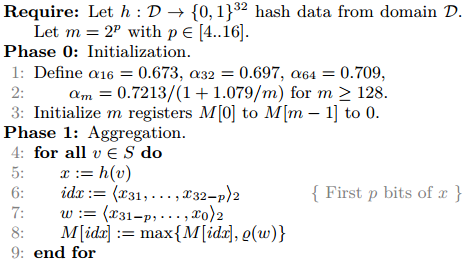
\includegraphics[scale=0.8]{HLL1.png}

\end{figure}
\end{frame}
\begin{frame}
\begin{figure}[H]
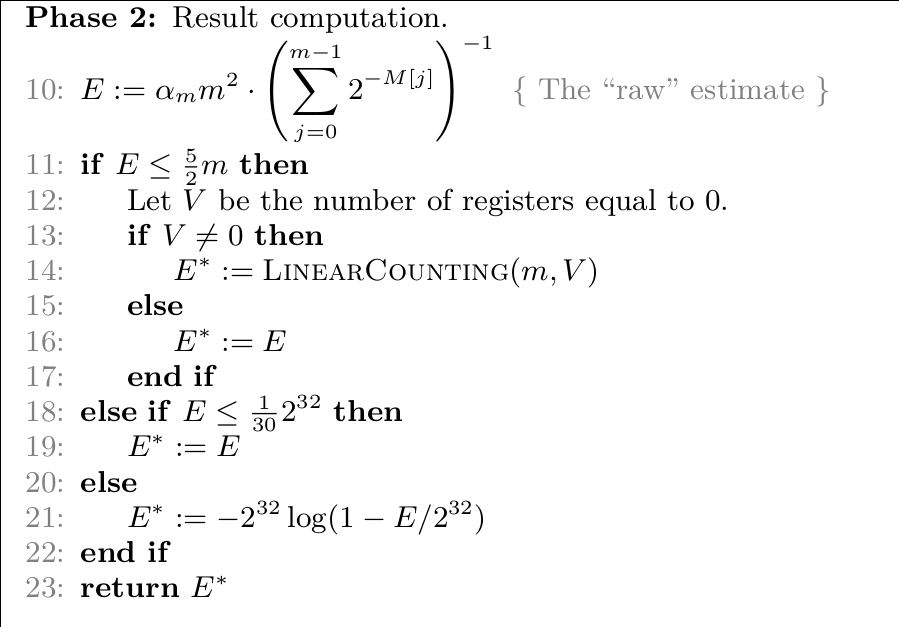
\includegraphics[scale=0.4]{HLL2.png}
\end{figure}
\end{frame}


\section{Các cải tiến cho HyperLogLog }
\begin{frame}{Các cải tiến cho HyperLogLog}

\end{frame}
\begin{frame}{Sử dụng hàm băm 64 bit}
\subsection{Sử dụng hàm băm 64bit}
\begin{itemize}
\item[•] Hàm băm L bits có thể có $2^L$ giá trị phân biệt. Nếu lực lượng của tập n có $2^L$ biểu diễn thì xung đột hàm băm có khả năng nhiều xảy ra $\rightarrow$ ước lượng chính xác là không thể.
\item[•] Yêu cầu bộ nhớ $\lceil log_2(L + 1 - p) \rceil .2^p$ bits
\begin{itemize}
\item L bits hàm băm, độ chính xác p.
\end{itemize}
\item[•] Sử dụng 64 bits yêu cầu bộ nhớ $6.2^p$
\begin{itemize}
\item không cần quan tâm xung đột hàm băm \\
(lực lượng tập $2^{64} \approx 1.8\cdot 10^{19}$ )
\item Large range correction là không cần thiết 
\end{itemize}
\end{itemize}
\end{frame}


\begin{frame}{Ước lượng cho tập lực lượng nhỏ(Estimating Small Cardinalities)}
\subsection{Ước lượng cho tập lực lượng nhỏ}
\begin{itemize}
\item[•] Với tập lực lượng nhỏ $HLL_{ORIG}$ cho kết quả tệ
\begin{itemize}
\item[•] Nếu n = 0,1,2 thuật toán luôn trả về $\approx 0.7m$ 
\end{itemize}
\item[•] Để đạt được ước lượng tốt cho tập lực lượng nhỏ
\begin{itemize}
\item $HLL_{ORIG}$ sử dụng LINEARCOUNTING khi $E < \frac{5}{2}m$
\end{itemize}
\end{itemize}
{\color{hilight} Nhận xét:} Kết quả không chính xác là do "độ lệch"\\
{\color{hilight} Giải pháp:}
\begin{itemize}
\item Hiệu chỉnh độ lệch
\end{itemize}
 $ \gg $ Hi vọng sẽ đạt được ước lượng tốt hơn nếu độ lệch được hiệu chỉnh đúng


\end{frame}
\begin{frame}{Các thử nghiệm}
\bi
\item Chay thuật toán $HLL_{64BIT}$ không sử dụng LINEARCOUNTING và đo ước lượng cho 1 khoảng với các lực lượng khác nhau
\bi
\item Ước lượng với $p = 14$ trên tập 5000 tập dữ liệu tạo ngẫu nhiên cho mỗi lực lượng
\item Sử dụng cùng 1 hàm băm 64 bit cho tất cả thực nghiệm.
\item Kiểm tra với nhiều hàm băm khác nhau (MD5, SHA256,MURMUR3)
\ei

\ei
{\color{hilight} Kết quả thử nghiệm:}  Chưa tìm dấu hiệu để hàm băm này thực hiện tốt hơn các hàm băm khác
\end{frame}
\begin{frame}{Hiệu chỉnh độ lệch theo kinh nghiệm}

\begin{figure}[h]
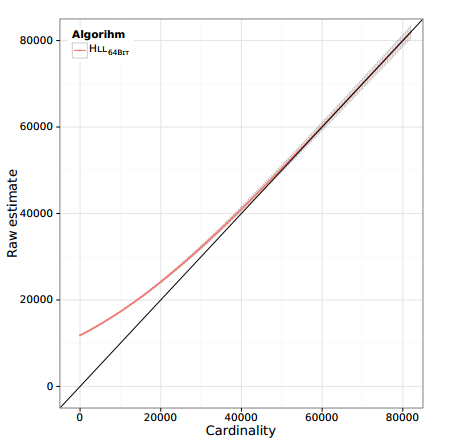
\includegraphics[scale=0.5]{img1.png}
\caption{Trung bình độ lêch thô của thuật toán $HLL_{64BIT}$}
\end{figure}
{\color{hilight} Nhận xét:}  $n > 5m$ hiệu chỉnh gần như là không  cần thiết
\end{frame}

\begin{frame}{Hiệu chỉnh độ lêch theo kinh nghiệm}
Chúng ta có thể tính toán các quan sát độ lệch và sử dụng nó để hiệu chỉnh ước lượng \\ 

Để làm trong thực tế:
\bi
\item Chọn 200 tập lực lượng khác nhau bởi các điểm nội suy
\item Ghi lại trung bình ước lượng thô và độ lệch(sai số).
\item Dùng k-nearest neighbor nội suy để lấy độ lệch cho một cái ước lược thô.(k = 6).
\ei
\end{frame}
\begin{frame}{Sử dụng thuật toán}
\begin{itemize}
\item Chạy thực nghiệm 3 thuật toán với các lực lượng khác nhau và so sánh phân bố error.
\bi
\item LINEARCOUNTING, bias-corrrected raw estimate, raw estimate.
\ei
\end{itemize}
\begin{figure}[h]
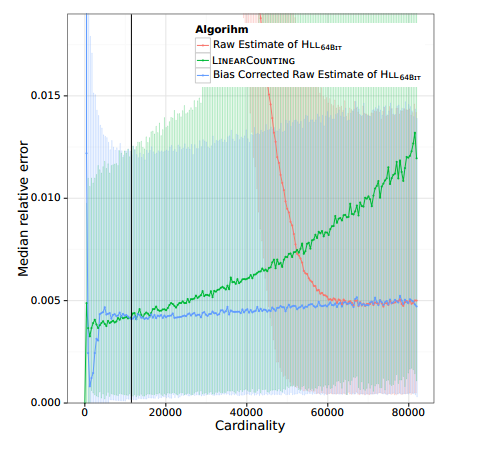
\includegraphics[scale=0.5]{img2.png}
\caption{Trung bình error của 3 thuật toán}
\end{figure}
\end{frame}
\begin{frame}{Ưu điểm của hiệu chỉnh độ lệch}
Sử dụng bias-corrected trộn với LINEARCOUNTING có ưu điểm hơn so với raw estimate trộn với LINEARCOUNTING.
\begin{itemize}
\item Lỗi cho 1 khoảng quan trọng của các lực lượng nhỏ hơn lỗi của $HLL_{64BIT}$
\item Kết quả của thuật toán không có độ lệch đáng kể.

\end{itemize} 
\end{frame}
\subsection{Biểu diễn thưa ( Sparse Representation )}
\begin{frame}{Biểu diễn thưa}
\bi
\item $Hll_{NoBias} $ yêu cầu bộ nhớ là 6m bit với bất kì n  \\
\item Trong trường hợp $n\ll m $ ta nhận thấy việc sử dụng bộ nhớ này hoàn toàn không hiệu quả \\
$ \gg$ Vì vậy trong trường hợp này ta nên sử dụng biểu diễn thưa ( Sparse Representation ), lưu các cặp $(idx,\varrho(w)) $ thành một danh sách thay vì sử dụng cả một mảng M như trước để tiết kiệm bộ nhớ\\
\item Chuyển giá trị cặp $(idx,\varrho(w)) $ thành một số nguyên bằng các biểu điễn thành một dãy bit trong đó idx là những bit cao và $\varrho(w) $ được lưu ở nhưng bit thấp\\
\ei
\end{frame}
\begin{frame}{}
\bi

\item Để tăng tốc độ ta sử dụng một tập tạm thời tập này sẽ trộn với danh sách ở một thời điểm nào đó(vd : 25 $\%$ của danh sách) \\


\ei
{\color{hilight} Nhận xét:} Vì các tập đã được sắp xếp theo idx nên khi trộn tập với danh sách ta chỉ cần duyệt một lần
\end{frame}
\begin{frame}{Lợi ích }
\begin{itemize}
\item Giảm không gian nhớ
\item Tăng một chút thời gian chạy với việc sử dụng tập tạm thời
\end{itemize}
\end{frame}
\begin{frame}{Tăng p với biểu diễn thưa} 
\bi
\item Trong biểu diễn thưa ta có thể chon p' >p (Precision) nó giúp ta tăng độ  độ chính xác của thuật toán lên.\\

\item Điều gì xảy ra nếu khi tăng p làm không gian lưu trữ vượt quá lên ngưỡng 6m bit.\\
\item Ta có thể chuyển một biểu diễn thưa với p' -> biểu điễn p bới thuật toán sau đây
\ei 
\end{frame}
\begin{frame}{Thuật toán chuyển độ chính xác}
Xét một cặp $(idx',\varrho(w)') $ với p' ta cần chuyển về $(idx,\varrho(w)) $ với p : 
\begin{figure}[H]
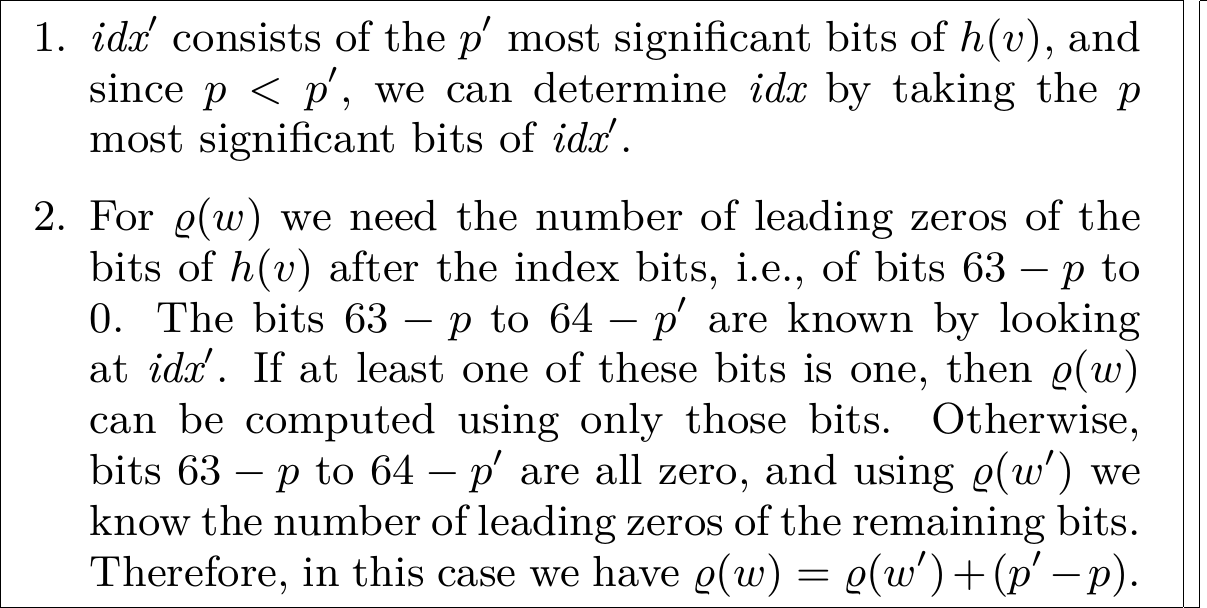
\includegraphics[scale=0.25]{HSR.png}
\caption {Thuật toán chuyển Precision}
\end{figure}

\end{frame}
\begin{frame}
\begin{figure}
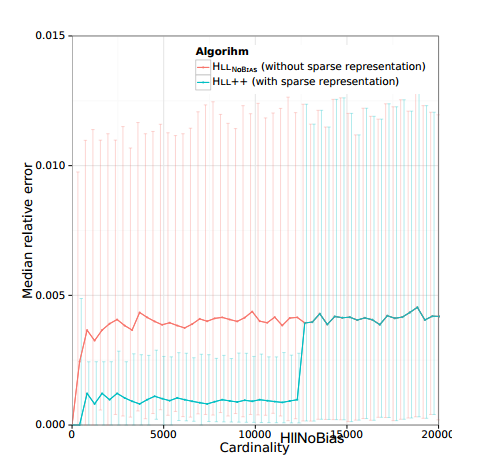
\includegraphics[scale=0.6]{img4.png}
\caption{So sánh Hll NoBias và  Hll++}
\end{figure}
\end{frame}
\begin{frame}{Giảm không gian nhớ với nén thưa }
\bi
\item Sử dụng biểu diễn nguyên cho $(idx,\varrho(w)) $ hoạt đông tốt nhưng một phần bit của bộ nhớ vẫn bị bỏ lãng phí.
\item Tuy nhiên ta có thể lưu ý 2 điều sau để dữ liệu lưu được đặc khít hơn:
\begin{itemize}
\item Sử dụng số nguyên với độ rộng cứng sẽ gây lãng phí
\item Danh sách cần được sắp xếp
\end{itemize}
\ei 
\end{frame}
\begin{frame}{Thực hiện}
\begin{itemize}
\item Chúng ta sẽ encode theo độ dài của biến
\item Ngoài ra chúng ta không lưu $a_1,a_2,a_3,...$ mà lưu $ a_1,a_2-a_1,a_3-a_2,...$\\

\end{itemize}

{\color{hilight} Nhận xét:} Khi nhìn vào việc thêm một phần tử vào danh sách nén ta sẽ thấy việc này khá là khó khăn nhưng xét trong một tiến trình trộn giữa tập tạm thời và danh sách nén thì việc này vẫn được thực hiện một cánh tuần tự.
\end{frame}

\begin{frame}{Nhận xét}
\bi 
\item Biểu diễn thưa thực chất chỉ đóng vai trò trong việc chuyển pha
\bi
\item Nhận thấy số lượng biến băm có thể lưu bằng biểu diễn thưa là nhỏ khi so ngưỡng chuyển từ Linear couting sang bias-corrected raw estimate  \\
\item Linear couting  chỉ yêu cầu m và số lượng các index tai đấy có giá trị nhớ bằng 0.\\
\ei
\ei
\end{frame}
\begin{frame}{Giảm không gian bộ nhớ cần lưu khi chuyển pha} 
Với các giá trị chuyển từ biểu diễn thưa lên biểu diễn thường:\\
{\color{hilight} Nhận xét:}\\
\bi
 \item $\varrho(w)$ chỉ cần lưu lại khi các bit $<x_{63-p} ,...,x_{64-p}>$ tất cả là 0
\item  Một hàm băm tốt thì xác suất lưu lại  $\varrho(w)$ $ 2^{p-p'}$
\ei 
{\color{hilight} Giải pháp:}
\\Thực hiện : sử dụng 1 bit đẻ cho biết ta có lưu lại $\varrho(w)$ không:
\begin{alltt}
 if $<x_{63-p} ,...,x_{64-p}>$ :tất cả là 0  $$<x_{63-p} ,...,x_{64-p}> || <\varrho(w)>||<1>$$
else $$<x_{63-p} ,...,x_{64-p}> ||<0>$$ 
\end{alltt}
\end{frame}
\begin{frame}{Hiệu quả không gian}
\begin{figure}[H]
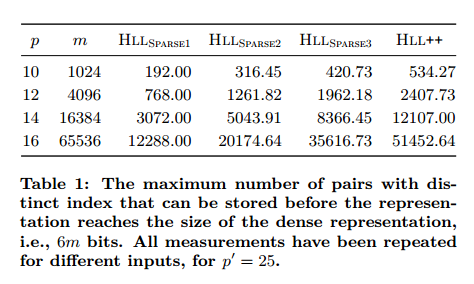
\includegraphics[scale=0.6]{img3.png}
\end{figure}
\begin{itemize}
\item $p = 14$ lưu mỗi phần tử trong biểu diễn thưa như 1 số nguyên sẽ cần 32 bit
\item Mã hóa thì điều này giảm 
\begin{itemize}
\item Độ dài trung bình 19.49 bits/phần tử
\end{itemize}
\end{itemize}
\end{frame}
\section{Kết luận}

\begin{frame}{Kết luận}
\begin{itemize}
\item $<12000$ sử dụng biểu diễn thưa đã làm giảm lỗi đáng kể
\item $12000\rightarrow61000$ sử dụng bias corection đã làm kết quả tốt hơn hẳn so với $HLL_{org}$
\item HLL++ tốn ít bộ nhớ hơn
\item Sử dụng hàm băm 64 bit cho phép ước lượng lên khoảng 1 tỉ
\end{itemize}

\end{frame}
\begin{frame}{Kết quả }
\begin{figure}[H]
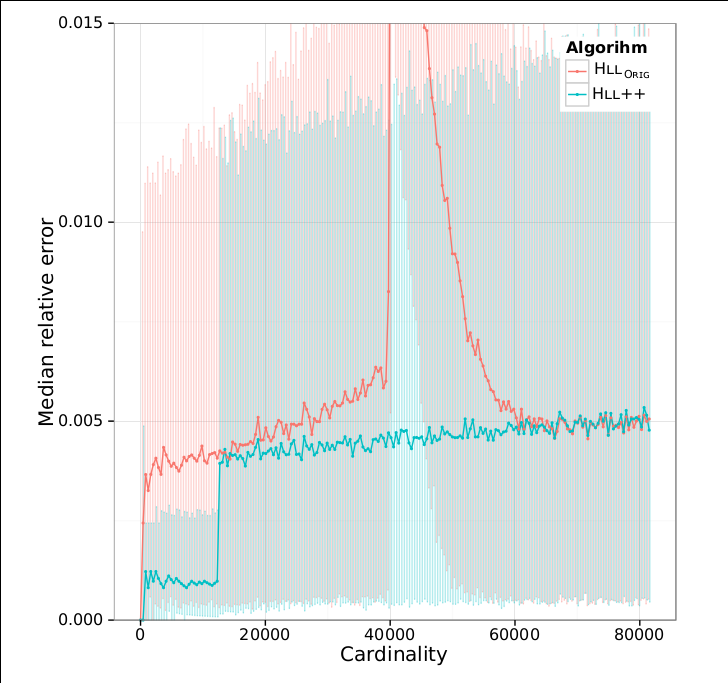
\includegraphics[scale=0.3]{KL.png}
\caption{ So sánh HLL và HLL++}
\end{figure}
\end{frame}
\section*{Tài liệu tham khảo}

% TODO: Book
\begin{frame}{Tài liệu tham khảo}
    \vspace{20pt}

    \bi
        \item HyperLogLog in Practice: Algorithmic Engineering of a
State of The Art Cardinality Estimation Algorithm by Stefan Heule Marc Nunkesser Alexander Hall
        \item Understanding the HyperLogLog: a
Near-Optimal Cardinality Estimation Algorithm
Philippe Flajolet, Èric Fusy, Olivier Gandouet and Frédéric Meunier
    \ei
\end{frame}

\begin{frame}
\includegraphics[scale=0.6]{thanks.jpg}
\end{frame}


\end{document}
